\documentclass[llncsdoc]{llncs}
\usepackage[latin1]{inputenc}
\usepackage{epsfig}
\usepackage{epstopdf}
\usepackage{graphicx}
\usepackage{makeidx}
\usepackage{subfigure}
\usepackage{multirow}
\usepackage{indentfirst}
\usepackage[printonlyused]{acronym}
\usepackage{booktabs}
\usepackage[table]{xcolor}
\definecolor{lightgray}{gray}{0.9}

\usepackage[table]{xcolor}
\usepackage{array}
\usepackage{url}
\newcolumntype{P}[1]{>{\centering\arraybackslash}p{#1}}
\begin{document}
\pagestyle{plain}
\makeatletter
\renewcommand\subsubsection{\@startsection{subsubsection}{2}{\z@}%
	{-18\p@ \@plus -4\p@ \@minus -4\p@}%
	{8\p@ \@plus 4\p@ \@minus 4\p@}%
	{\normalfont\normalsize\bfseries\boldmath
		\rightskip=\z@ \@plus 8em\pretolerance=10000 }}
\DeclareRobustCommand{\rchi}{{\mathpalette\irchi\relax}}
\newcommand{\irchi}[2]{\raisebox{\depth}{$#1\chi$}}
		
\title{Reputation Vault}


\author{João Santos\\joao.marques.santos@tecnico.ulisboa.pt}
\institute{Instituto Superior T�cnico\\(Advisors: Professors Nuno Santos and David Dias)}
\maketitle
\thispagestyle{plain}


\begin{abstract}

  Something about this
\end{abstract}

\section{Introduction}

\subsubsection{Understanding Reputation}


\subsubsection{Blockchain}
Blockchain technology was made popular with the creation of the Bitcoin \cite{Anonymous:JOJGrvgg}, in 2009. Bitcoin was the first truly decentralised crypto-currency, it uses cryptographic properties to solve the Double-spending problem and allows for parties to engage in transactions without having to trust each other. On backbone of Bitcoin is the blockchain which is a distributed ledger that keeps track of every valid transaction that ever took place in the network. Transactions are validated and packed into blocks that are then added to the ledger by nodes (miners) that run a consensus protocol, proof-of-work in the case of Bitcoin. Bitcoin's blockchain has full auditability \footnote{meaning that any node can verify the validity of any transaction} and correctness \footnote{meaning that all the transactions on the longer chain are valid}.

Following Bitcoin's success, a large and active community has emerged and worked on a lot of modifications and extensions to the original protocol to improve some of Bitcoin's shortcomings like performance, introduce new consensus protocols, add new features. These modifications and extensions, which are usually forks of Bitcoin or abstractions that sit on top of existing blockchains, are called "alt-coins", \cite{Bonneau:2015ema}.

// // Aqui falar mais sobre alt-coins // //

One of the shortcomings of Bitcoin was the lack of contract customisation as while it did allow for parties to create some rules regarding a given transaction (such as requiring a third party to approve the transaction) doing so required learning a not very intuitive scripting language and functionality was extremely limited. In other words, it only allowed for a very simple form of smart contracts \footnote{smart-contracts are programs that run on the blockchain and allow for the creation of special transaction rules}. Ethereum is a crypto-currency blockchain, similar to Bitcoin in many ways, that is a smart contract and decentralised application platform. It has a Turing complete programming language which allows for users to create distributed applications while making use of the features of the blockchain.

\subsubsection{Where Reputation and Blockchain Meet}
Blockchains such as Bitcoin or Ethereum are truly decentralised systems that ensure correctness. They can not be controlled by one single party and all the state transitions they store can be audited by any node. Ethereum's smart contracts and programmability features can be leveraged to create a decentralised reputation system that provides the same functionality as current systems, such as eBay's or LinkedIn's, while solving the information silo problem. It allows for each node to have control over its identity and know that the system will never cease to exist. There are currently some blockchain reputation systems that aim at doing this, \cite{Dennis:2016um}, \cite{Yasin:2016ja} and \cite{Buechler:2015tv}. At the same time, communities have formed pursuing efforts in this field, like Rebooting The Web of Trust and IDEO CoLab's Mosaic, that focuses mainly on identity.



\section{Goals}
\label{sec:goals}

This project serves one purpose.
 
\begin{quotation} 
\textit{Goals:} To create an amazing system.
\end{quotation} 
 
\begin{quotation} 
  \textit{Expected results:} Be hired by and become best friends with Elon Musk.
\end{quotation} 

\section{Related Work}
\label{sec:rwork}

\subsubsection{Types of Reputation Systems}
Centralised vs distributed
Reputation Algorithms



\subsubsection{Identity and Reputation}
One of the keys to having a good reputation system is having a strong identity framework put in place. As we are going to see later, many of the deficiencies of current reputation systems originate in poor identity verification mechanisms operating on the backbone of said reputation systems. It is essential to ensure that one person is linked to one and only one identity.

\subsubsection{Silos and Walled Gardens}
Many of the identity and reputation systems (Google, Facebook, Amazon) we use today are extremely atomic in the sense that the information collected by each one is not shared, or even compatible, to the one that is stored in other systems. What this creates, for each user, is a set of incomplete identities. Each platform only looks to a subset of features of a user and that prevents it from creating a holistic picture of him. In places like Amazon and eBay we have what is called an identity silo \cite{Pato:2017uw}, where the information in centralised and controlled by one entity without the possibility of being interchanged with another platform that might serve a similar purpose. Google and Facebook also started off as being identity silos, but now with the single sign on features \cite{Anonymous:MGy1lR79} they became what are known as Walled Gardens \cite{Pato:2017uw}, which are like Silos but that allow some information to be shared with some other organisations. \cite{Anonymous:PvP3cFwB} and \cite{Mostarda:2009te} suggest a solution to part of this problem in the form of a social network's social graphs aggregator. 

\subsubsection{Reputation Systems Attacks and Vulnerabilities}
\cite{Hoffman:2009gm} suggests a classification of these attacks in five categories. 
\begin{itemize}
     

\item Self-promoting, where attackers falsely increase their own reputation
\item Whitewashing, where attackers leverage system vulnerabilities to repair their reputation, effectively giving themselves a clean slate to continue engaging in malicious behaviour.
\item Slandering, where attackers lower other users' reputation score by illegitimately (without having existed an interaction) rating them.
\item Orchestrated, where several attackers collude to carry on one of the attacks described above.
\item Denial of service, where attackers prevent the calculation and dissemination of reputation scores thus compromising the normal function of the system.
\end{itemize}

\subsection{Bitcoin}

\subsubsection{Historical Context}

 Since the 1980's that there had been proposals for crypto-currency systems and in 2005 for decentralised consensus protocols. The proposed crypto-currency systems were never widely adopted due to the need of a centralised platform, as for the decentralised consensus protocols, they never became a reality as it was unclear how to carry out the implementation.
 Bitcoin's white paper,\cite{Anonymous:JOJGrvgg}, was published in 2009 by Satoshi Nakamoto (a pseudonym) and it was the first successful implementation of a decentralised cryptocurrency system.
 
 The technical breakthrough it provided was the implementation of a blockchain, a distributed ledger that keeps track of transactions. 
 \subsubsection{Technical Breakthrough}
 Bitcoin proposed an alternative mode of establishing trust between transacting parties. On traditional financial transaction systems, such as banks, two transacting entities have trust on a centralised element, the bank. Let us look at the example of a normal wire-transfer. User A sends money to user B. Both A and B are confident that the bank will withdraw the right amount of money from A's account and place that same amount in B's account. In this traditional trust model the bank is an essential entity in the process as it constitutes the only source of trust between the two transacting parties. Bitcoin's approach is different. Instead of asking the two parties to trust each other, it uses a proof-of-work system whose cryptographic properties are enough to assure transactional correctness as long as honest nodes control the majority of the CPU power of the network.
 
 An electronic currency is nothing more than a piece of digital data and one of the features of digital data is their easy replication. For that reason, an issue that an electronic currency has to tackle is the double spending problem. That is, ensuring that a given node is not able to spend the same token\footnote{coin, a unit of digital currency} more than once. The way to solve this problem without resorting to a centralised system is to create a ledger of transactions and get all the nodes to agree on the content of that ledger. 
 To that end, a consensus protocol is used, the Bitcoin consensus protocol, also known as the Nakamoto Consensus if based on a proof-of-work.
 
 \subsubsection{Transactions and Proof-of-Work}
 A Bitcoin transaction consists on nodes exchanging unspent coins and is identified by chain of digital signatures. To complete a transaction the sending node digitally a hash that identifies the past transaction and the public key of the next owner. This ensures that each transaction is linked to the ones preceding it, creating a chain.
 The next key challenge is getting all the nodes to agree on the set of past transactions, in order to prevent double-spending.
 To that end transactions are packed into blocks, and added to an append-only data structure, the blockchain.
 
 To add a block to the blockchain, nodes have to mine the block and the way to do that is to solve a mathematical challenge with a pre-defined difficulty level. The first node to solve that challenge mines the block, permanently adding it to the Blockchain. Each time a node mines a block, a new Bitcoin (coin) is created and given to that node. This constitutes an incentive for nodes to mine. The algorithm is designed to automatically adjust the challenger's difficulty in order to regulate the currency issuing rate.
 
 All the mined blocks are made of transactions that are linked to each other, which means that if a dishonest node was to change a past transaction that change would be eventually be detected by an honest node.
 
 
\subsubsection{Solving Forks}
Sometimes a node will mine a block that has already been mined by another node but due to network latency the first is unaware of this. In this situation a fork occurs. Both of these blocks are propagated through the network and eventually a new block will be mined and appended to one of those forks. The network will chose the longest fork as the standing one.

\subsection{Ethereum}
The alt-coins seen in \ref{alt-coins} aim at solving some of bitcoin's shortcomings and lack of functionality, however they are highly optimised for one use case and lack flexibility to serve other purposes. Ethereum aims at solving this by offering smart-contracts \footnote{A script that runs in the blockchain} that have Turing completeness, effectively offering a state-machine that runs on the blockchain.

Ethereum is built on many of the same principles as Bitcoin. Is is a blockchain based system that can also serve as a cryptocurrency. It also uses a proof-of-work mechanism as consensus protocol, albeit with a difference, while Bitcoin's consensus protocol challenge lies on CPU power, Ethereum's lies on memory requirement. The goal of this different implementation is to make the network more democratic. One of the consequences of Bitcoin's consensus protocol was the creation of mining farms\footnote{Infrastructures provided with bitcoin mining specialised hardware} which resulted on an uneven distribution of the mining power among active nodes. Memory is something that is extremely optimised on pretty much every electronic device nowadays, much more than CPU power, so this measure should empower lighter miners to the detriment of more powerful ones.

\subsubsection{Turing Completeness}
Ethereum allows for developers to apply arbitrary logic to smart-contracts. Its transactions can be of one of two types.
\begin{itemize}
    \item Private: Are controlled by an ECC\footnote{Elliptic curve cryptography} private key and allow for currency transaction.
    \item Smart-contract: These are transactions controlled by the logic programed into a smart contract.
\end{itemize}
Both types of transactions can interact with one another (a private transaction can interact with a smart contract and the latter can also engage with a private transaction).
From a programing stand point, one can look at smart-contracts as objects in the Ethereum universe, these objects can interact with each other to fulfil any business rules required by an application.

A smart-contract has to define an upper limit of computing power it will use, this limit of computing power is knows as Gas. The amount of Gas a program has is what defines for how long it can be ran by Ethereum nodes. Gas costs money and miners are rewarded with that Gas. This condition is extremely important to stop programs that halted and malicious programs designed to enter an infinite loop. If a program runs and terminates successfully and does not spend all the Gas, the remainder is returned to the smart-contract, and can be used in future executions. On the other hand if a smart-contract runs out of Gas before ending its execution, all the changes made by the smart-contract are rolled back (to prevent inconsistent states) but the Gas is not returned to the smart-contract, it is given to the miners.

\subsection{Verity}

Verity is a very ambitious blockchain based reputation system. It offers a general reputation repository for both users and content. Its reputation system is to serve as a base for crowd-sourcing platforms, and governance. A users reputation is divided into values and technical skills. 

\subsection{IPFS}

\subsection{Open Badges}

\subsection{Blockcerts}

\begin{figure}
  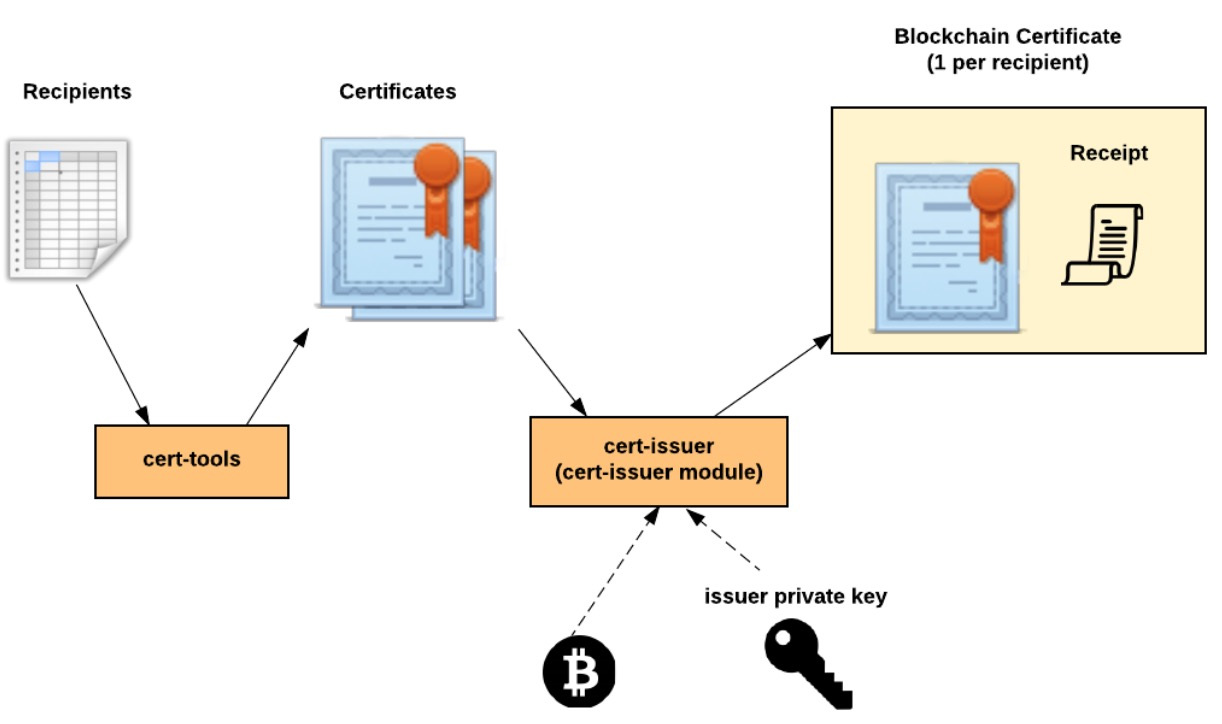
\includegraphics[width=\linewidth]{figures/blockcerts_arch.jpg}
  \caption{Blockcerts' Architecture}
  \label{fig:blockcerts_arch}
\end{figure}

\subsubsection{Certificate Revocation}
\label{revoked}
One can think of a number of reasons a certificate may be revoked and as of now the way an Issuer can revoke a certificate it emitted if by publishing said certificate's ID on a Revoked Certificates List (each certificate has a field that says where to obtain the issuer's list of revoked certificates). This raises several problems, both from a technical perspective as well as a privacy one.

%%%%%%%%%%%%%%%%%%%%%%%%%%%%%%%%%%%%%%%%%%%%%
\section{Proposed Solution}
This body of work is going to address two issues: 
\begin{enumerate}
    \item Certificate Revocation
    \item Issuer Storage Dependency
\end{enumerate}

To address the first we propose a new certificate revocation technique that leverages smart-contracts to remove the need for Revoked Certificates Lists and to address the second we propose a new method to store certificates that relies on the distributed file system, IPFS.


\subsection{Certificate Revocation}
\label{cert_revocation}
Blockcerts follows OpenBadges' specification for certificates revocation method. As of now, the way this is done is by having the issuer maintain a list of revoked certificates. An address to that list is provided on each issued certificate so that any party who wants to check the state of the certificate can do so by cross checking the certificate's ID with the list of revoked certificates.

This approach has been discussed in Blockcerts' forum and several problems have been highlighted:
\begin{itemize}
    \item \textbf{The issuer has total control over the certificate-} The certificate can only be revoked by the issuer (as he is the one in control of the revoked certificates list) and in the case of there being a need to revoke a batch of certificates, it has to be done one by one.
    \item \textbf{Verification relies on a third party-} Since the list is kept by the issuer, each time a party wants to verify a certificate it will have to communicate with the issuer. This creates a perpetual dependency between each certificate and its issuer which in turn defeats some of the purposes of using a blockchain, namely the capability of having a decentralised perpetual correct ledger. If the issuer ceases to exist there is no longer a way to revoke the certificates it once issued. This issue also ties up
    \item \textbf{Raises privacy concerns-} Each time the certificate revocation list is consulted on can assume the issuer can know about it (since it is the one hosting the list). This informs the issuer about the way the certificates are being used. Moreover, for each revoked certificate in that list there is a field in which the issuer can clarify the reason for the revocation, since the revoked certificates list is public, anyone can crawl those lists gathering information about revoked certificates.
  
\end{itemize}

There are several ideas on how to solve this. One proposed approach is to use Bitcoin's unspent transaction outputs (UTXOs). By assigning and UTXO to a certificate the way to revoke said certificate would be to perform a transaction that utilised that UTXO, which would render the unspent transaction output, spent. This approach solves all the problems that come with the Revoked Certificates List. The certificate can now be revoked by more than one party (by implementing a Bitcoin smart-contract with multi-signature), the verification no longer requires a third party, as it can be made entirely relying on the Bitcoin blockchain and privacy concerns are no longer an issue (certificate revocation reasons are still public but are recorded i individual files, rather than being all together on a list).

Even though this mechanism would solve the problems with the existing system, it also adds problems of its own:
\begin{itemize}
    \item \textbf{Provides little functionality-} Once revoked the certificate can no longer the valid. A desirable feature on a system such as this one would be the ability to freeze certificates, that same way bank accounts can temporarily be frozen.
    \item \textbf{It is Bitcoin specific-} Even though Blockcerts' current implementation is made on top of the Bitcoin blockchain, the long-term goal is for it to be blockchain agnostic. For that reason, creating a dependency on the Bitcoin blockchain is not a desirable feature.
    \item \textbf{The cost of revoking batches if very high-} It is legitimate to assume that sometimes there will be the need to revoke a batch of certificates. With this approach this would require one transaction per revoked certificate. Since each transaction has a cost associated with it, revoking a whole batch of certificates would make the revoking cost grow linearly with the number of certificates in the batch.
\end{itemize}

\subsection{Our approach}
Our proposal is to leverage Ethereum's smart contracts to handle certificate revocations. This would allow us to add a lot of functionality and flexibility to the system.
\subsubsection{Scope}
It is important to mention that this would not automatically solve the issue of dependence on a specific blockchain. That is outside of the scope of this work. There is a proposal to how that should be address and it points towards there being an implementation per blockchain (one for Bitcoin, one for Ethereum, etc) and then having Blockcerts interface with them. So even though this does not make Blockcerts blockchain agnostic, it contributes to the effort of having an implementation per blockchain. This is illustrated in \ref{fig:scope}

\begin{figure}
  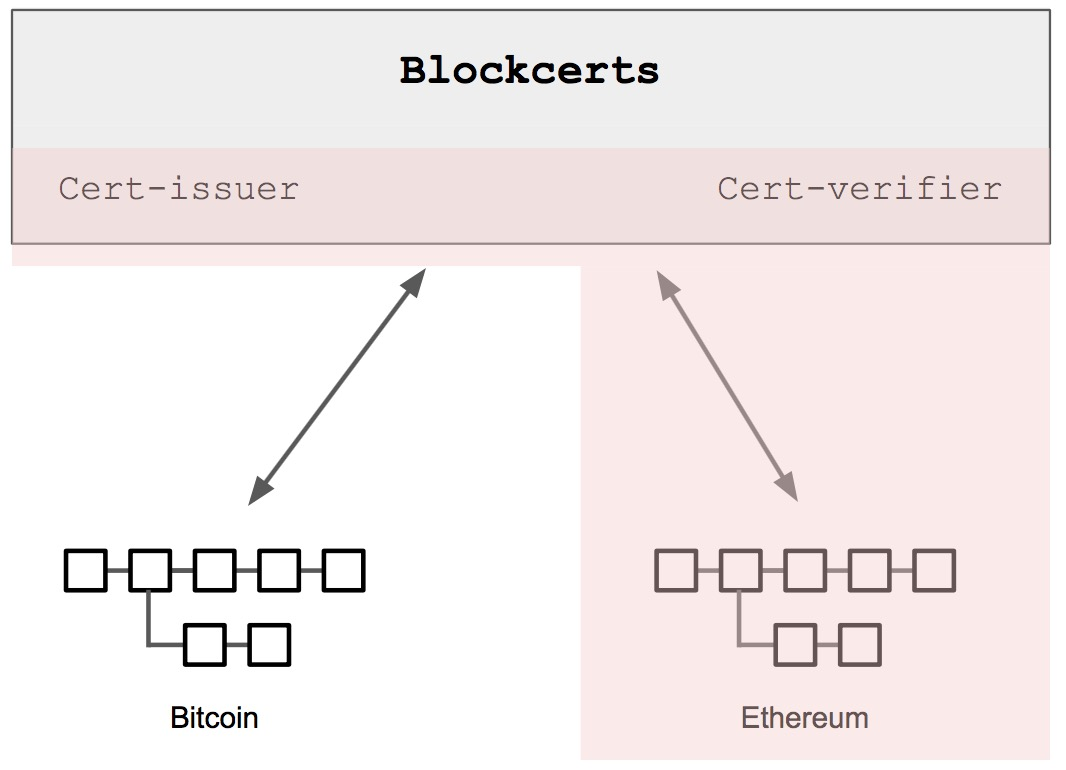
\includegraphics[width=\linewidth]{figures/arch.jpg}
  \caption{Scope of this work. We will focus on developing an Ethereum smart-contract's implementation for certificate revocation}
  \label{fig:scope}
\end{figure}
\subsubsection{Functionalities}
Our implementation will support the following functionalities, which were suggested in  Blockcerts' forum as desirable features, to the certificate revocation mechanism:
\begin{itemize}
    \item \textbf{Revocation by the Issuer-} Just like it currently exists.
    \item \textbf{Revocation by the Receiver-} A new functionality, not supported by revoked certificates list, which gives the receiver full control over the certificates it may hold. It is legitimate to imagine a scenario where a receiver no longer wants to be associated with a given Issuer.
    \item \textbf{Revocation by a third-party-} Another new feature which will allow a third-party, authorised by the Issuer and Receiver, to revoke a certificate.
    \item \textbf{Revocation by a combination of Issuer, Receiver and third-party}
    \item \textbf{Temporary revocation} A unique feature of a smart-contract based approach to this is that the revocation status can be changed over time. This will allow for temporary revocation status that can be triggered by a programmable action (for instance, a certificate can be revoked if a receiver fails to pay a pre-accorded monthly fee).
    \item \textbf{Batch revocation-} This implementation will allow for an easy batch revocation.
\end{itemize}

\subsubsection{Implementation}
Ethereum offers a great set of tools that will enable us to add aforementioned functionalities to the system. Since it's Turing complete and has support for familiar programing languages, its smart-contracts can be programmed almost like normal applications.

The revocation status of a given certificate can be maintained as a variable in a smart-contract. Certificates revocation status can be accessed individually or as a batch. A simple architecture to support this would be to have a smart-contract per batch of certificates. 

Implementing an Ethereum smart-contracts solution for certificate revocation will require changes to some of Blockcerts' components (refer to Figure \ref{fig:blockcerts_arch}):
\begin{itemize}
    \item \textbf{Blockcerts Schema-} The Blockcerts schema defines the fields and schema a certificate must have in order to be Blockcerts compliant. Currently one of the required fields is the Revocation List, which contains either an HTTP URI\footnote{Uniform Resource Identifier} pointing towards the Issuer's revoked certificates list or an embedded array of revoked certificates. This schema will be extended in order to contain a URI pointing towards that specific certificate's status, that URI can point to an Ethereum smart-contract, to a Bitcoin UTXO, depending on the implementation (this because even though we will be procuring an Ethereum implementation, the goal is to make Blockcerts certificate revocation function with any blockchain that can support the functionality).
    
    \item \textbf{Cert-Tools-} This component receives inputs\footnote{Data relevant to the issuing of the certificate} from the Issuer and outputs a Blockcerts compliant certificate.It will be required to extend this component to comply with the schema changes proposed above.
    \item \textbf{Cert-Verifier-} The Cert-verifier is responsible for checking the integrity, authenticity and revocation status of a given certificate. This component will also be extended to account for the new revocation status verification mechanism. In this case it will check the revocation status in the Ethereum smart-contract.
\end{itemize}

\subsection{Remove dependencies from issuers' storage}
In the current implementation of blockcerts, the Issuers are the ones responsible for keeping a copy of the certificates. This not only creates a single point of failure but also, just like the revoked certificates list case, creates a perpetual dependency on the Issuer. IPFS offers an efficient distributed storage solution. Contents are addressed by unique links that are permanent and immutable.

Blockcerts provides a reference mechanism for Issuers to store their issued certificates, Cert-store, which is implemented in MongoDB. They do make clear, however, that this implementation is not part of the standard and that any Issuer can have different approaches to how they store their certificates. The only required aspect is that the certificates can be retrieved via a URL, and IPFS complies with that.

In order to accomplish certificate storage on IPFS we propose to change the Cert-store and the Cert-viewer.
\begin{itemize}
    \item \textbf{Cert-Store:} This is the application that Issuers can use to store their issued certificates. We want to implement this application in a way that stores certificates on IPFS.
    \item \textbf{Cert-viewer:} This application is used to retrieve certificates when provided with a URL. We need to extend this application in order to support IPFS' URLs.
\end{itemize}


\section{Evaluation}
\label{sec:evaluation}
\begin{itemize}
    \item Cost vs current system: can be done with private ethereum blockchain implementations
    \item time to revoke batches: has to be testes in the real blockchain
    \item functionality
\end{itemize}

\subsection{Performance Evaluation}

\section{Scheduling of Future Work}
\label{sec:fwork}

Future work is scheduled as follows:

\begin{itemize}
\item \textbf{September 15 - December 10} 
    \begin{itemize}
        \item Detailed design specifications, implementation and documentation.
        \item Submit the software to Blockcerts' Github repository as a pull request.
    \end{itemize}
\item \textbf{December 10 - January 5}
    \begin{itemize}
        \item Receive community feedback and improve the solution. 
        \item Start writing a technical paper describing the solution. 
        \item Start system evaluation.
    \end{itemize}
\item January 5 - : Write a paper describing the project.
\item May 24 - June 15: Finish the writing of the dissertation.
\item February 20: Deliver the MSc dissertation.

\end{itemize}

\section{Conclusions}
\label{sec:conclusions}



\bibliographystyle{splncs}
\bibliography{relatorio}

\acrodef{IDK}{I Don't Know}

\end{document}
